\section{Low-Voltage Induced Random Bit Errors in Quantized DNN Weights}
\label{sec:errors}

We assume the quantized DNN weights to be stored  on multiple memory banks, \eg, SRAM in the case of on-chip scratchpads or DRAM for off-chip memory. As shown in \cite{GanapathyDAC2017,KimDATE2018,ChandramoorthyHPCA2019}, the probability of memory bit cell failures increases exponentially as operating voltage is scaled below $\Vmin$, \ie, the minimal voltage required for reliable operation, see \figref{fig:introduction}. This is done intentionally to reduce energy consumption, \eg, \cite{ChandramoorthyHPCA2019,KimDATE2018,KoppulaMICRO2019}, or adversarially by an attacker, \eg, \cite{TangUSENIX2017}. Process variation during fabrication causes a variation in the vulnerability of individual bit cells. As shown in \figref{fig:errors} (left), for a specific memory array, bit cell failures are typically approximately random and independent of each other \cite{GanapathyDAC2017}. We also consider chips showing other error patterns as in \figref{fig:errors} (right). Nevertheless, there is generally an ``inherited'' distribution of bit cell failures across voltages \cite{GanapathyHPCA2019}, if a bit error occurred at a given voltage, it is likely to occur at lower voltages, as made explicit in \figref{fig:errors}. However, across different SRAM arrays in a chip or different chips, the patterns or spatial distribution of bit errors is usually different and can be assumed random \cite{ChandramoorthyHPCA2019}. Throughout the paper, we use the following bit error model:

\textbf{Random Bit Error Model:}
\textit{The probability of a bit error is $p$ (in \%) for all weight values and bits. For a fixed memory array, bit errors are persistent across supply voltages, \ie, bit errors at probability $p'{\leq}p$ also occur at probability $p$. A bit error flips the currently stored bit. We denote random bit error injection by $\biterror_p$.}

\begin{figure*}
    \vspace*{-0.15cm}
    \centering
    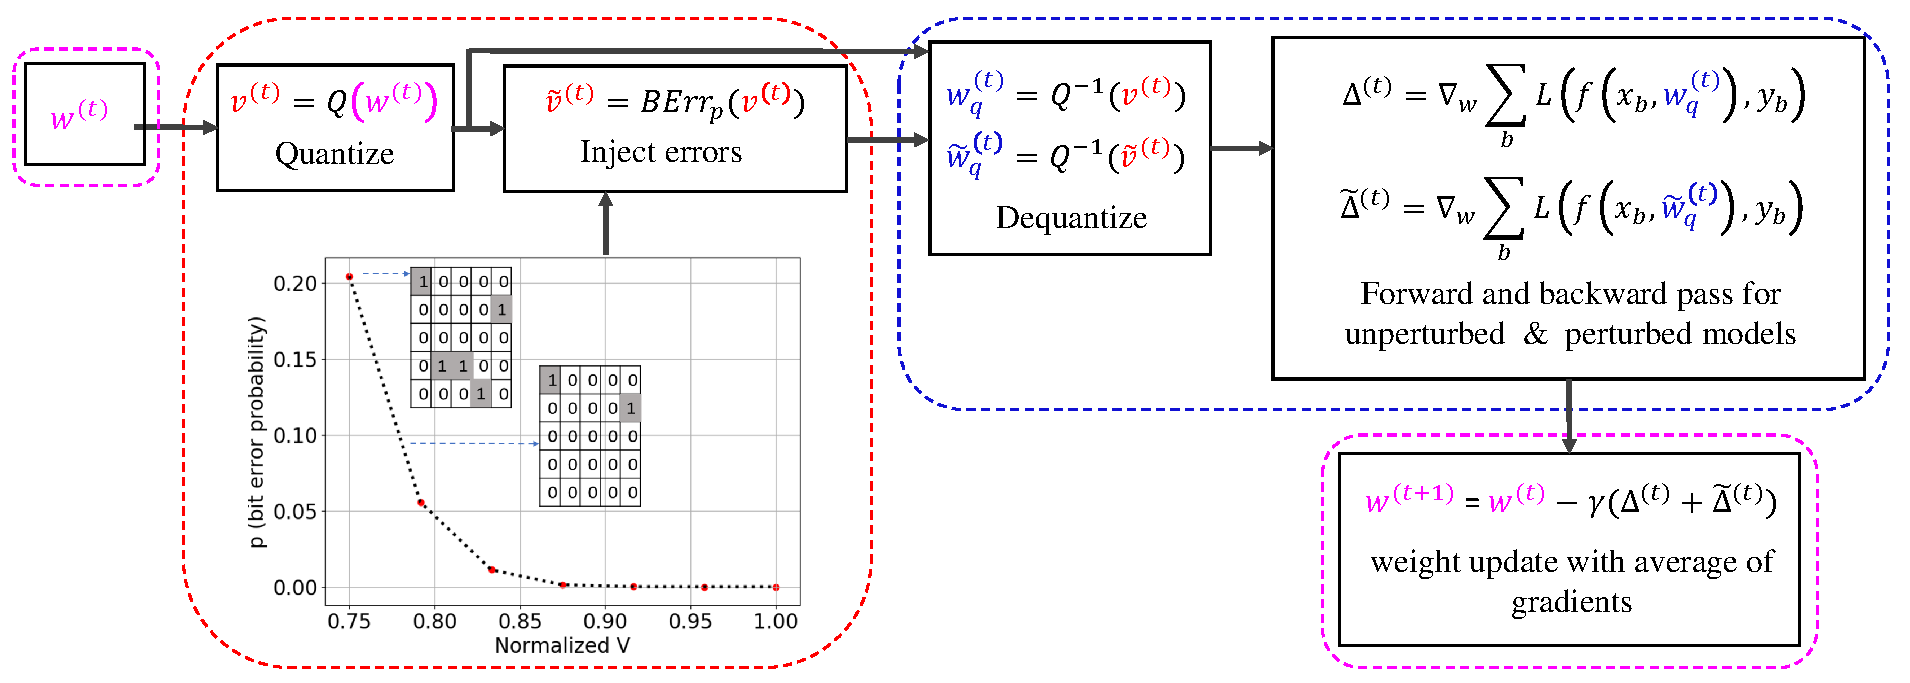
\includegraphics[width=0.85\textwidth]{main_training_flow4.pdf}
    \vspace*{-6px}
    \caption{\textbf{Random Bit Error Training (\Random).} We illustrate the data-flow for \Random as in \algref{alg:training}. Here, $\biterror_p$ injects random bit errors in the \red{quantized weights} $\red{v^{(t)}} = Q(\magenta{w^{(t)}})$, resulting in $\red{\tilde{v}^{(t)}}$, while the forward pass is performed on the \blue{de-quantized perturbed weights} $\blue{\tilde{w}_q^{(t)}} = Q^{-1}(\red{\tilde{v}^{(t)}})$, \ie, fixed-point arithmetic is not emulated. The weight update during training is not affected by bit errors and computed in \magenta{floating point}.}
    \label{fig:flowchart}
    \vspace*{-0.2cm}
\end{figure*}

This error model realistically captures the nature of low-voltage induced bit errors, from both SRAM and DRAM as confirmed in \cite{ChandramoorthyHPCA2019,KimDATE2018,KoppulaMICRO2019}. However, our approach in \secref{sec:robustness} is model-agnostic: the error model can be refined if extensive memory characterization results are available for individual chips. For example, faulty bit cells with $1$-to-$0$ or $0$-to-$1$ flips might not be equally likely. Similarly, as in \cite{KoppulaMICRO2019}, bit errors might be biased towards alignment along rows or columns of the memory array. The latter case is illustrated in \figref{fig:errors} (right). However, estimating these specifics requires testing infrastructure and detailed characterization of individual chips. 
More importantly, it introduces the risk of overfitting to few specific memories/chips. 
Furthermore, we demonstrate that the robustness obtained using our uniform error model generalizes to bit error distributions with strong spatial biases as in \figref{fig:errors} (right).

We assume the quantized weights to be mapped linearly to the memory. This is the most direct approach and, in contrast to \cite{KoppulaMICRO2019}, does not require knowledge of the exact spatial distribution of bit errors. This also means that we do not map particularly vulnerable weights to more reliable memory cells, and therefore no changes to the hardware or the application are required. Thus, in practice, for $W$ weights and $m$ bits per weight value, we sample uniformly $u \sim U(0, 1)^{W \times m}$. Then, the $j$-th bit in the quantized weight $v_i = Q(w_i)$ is flipped iff $u_{ij} \leq p$.
Our model assumes that the flipped bits at lower probability $p' \leq p$ are a subset of the flipped bits at probability $p$ and that bit flips to $1$ and $0$ are equally likely. The noise pattern of random bit errors is illustrated in \figref{fig:quantization}: 
for example a single bit flip in the most-significant bit (MSB) of the signed integer $v_i$ can result in a change of roughly half of the quantized range (also \cf \secref{subsec:robustness-quantization}).

\section{Towards Robustness Against Random Bit Errors}
\label{sec:robustness}

We address robustness against random bit errors in three steps: First, we analyze the impact of fixed-point quantization schemes on bit error robustness. This has been neglected both in prior work on low-voltage DNN accelerators \cite{KimDATE2018,KoppulaMICRO2019} and in work on quantization robustness \cite{MurthyARXIV2019,MerollaARXIV2016,SungARXIV2015}. This yields our \textbf{robust quantization} (\secref{subsec:robustness-quantization}). On top, we propose aggressive \textbf{weight clipping} as regularization during training (\secref{subsec:robustness-clipping}). 
Weight clipping enforces a more uniformly distributed, \ie, redundant, weight distribution, improving robustness. We show that this is due to minimizing the cross-entropy loss, enforcing large logit differences.
Finally, in addition to robust quantization and weight clipping, we perform \textbf{random bit error training (\Random)} (\secref{subsec:robustness-training}): in contrast to the fixed bit error patterns in \cite{KimDATE2018,KoppulaMICRO2019}, we train on completely \emph{random} bit errors and, thus, generalize across chips and voltages.
Generalization is measured using \emph{average robust test error (\RTE)}, the test error after injecting bit errors, \wrt to our error model from \secref{sec:errors} as well as real, profiled bit error patterns. % but also the corresponding standard deviation. 
Robustness against bit error rate $p$ has to induce robustness for $p' \leq p$ (\ie, higher voltage), as well.

\subsection{Robust Fixed-Point Quantization}
\label{subsec:robustness-quantization}

We consider quantization-aware training \cite{JacobCVPR2018,KrishnamoorthiARXIV2018} using a generic, deterministic fixed-point quantization scheme commonly used in DNN accelerators \cite{ChandramoorthyHPCA2019}. However, we focus on the impact of quantization schemes on robustness against random bit errors, mostly neglected so far \cite{MurthyARXIV2019,MerollaARXIV2016,SungARXIV2015}. We find that quantization affects robustness significantly, even if accuracy is largely unaffected.

\textbf{Fixed-Point Quantization:} Let $f(x; w)$ be a DNN taking an example $x \in [0, 1]^D$, \eg, an image, and weights $w \in \mathbb{R}^W$ as input. Quantization determines how weights are represented in memory, \eg, on SRAM. In a \emph{fixed-point quantization} scheme, $m$ bits allow to represent $2^m$ distinct values. 
A weight $w_i \in [-\qmax, \qmax]$ 
is represented by a signed $m$-bit integer $v_i = Q(w_i)$ corresponding to the underlying bits. Here, $[-\qmax, \qmax]$ is the \emph{symmetric} quantization range and signed integers use two's complement representation. Then, $Q: [-\qmax, \qmax] \mapsto \{-2^{m - 1} - 1, \ldots, 2^{m - 1} - 1\}$ is defined as 
\begin{align}
    Q(w_i) = \left\lfloor \frac{w_i}{\Delta}\right\rfloor,\text{  }
    Q^{-1}(v_i) = \Delta v_i,\text{  }
    \Delta = \frac{\qmax}{2^{m - 1} - 1}
    \label{eq:quantization}
\end{align}
Flipping the most significant bit (MSB, \ie, sign bit) leads to an absolute error of half the quantization range, \ie, $\qmax$ ({\color{yellow!75!black!}yellow} in \figref{fig:quantization}).
Flipping the least significant bit (LSB) incurs an error of $\Delta$, \cf \eqnref{eq:quantization}. Thus, the impact of bit errors ``scales with'' $\qmax$.

\textbf{Global and Per-Layer Quantization:} $\qmax$ can be chosen to accommodate all weights, \ie, $\qmax = \max_i |w_i|$. This is called \emph{global} quantization. However, it has become standard to apply quantization \textit{per-layer} allowing to adapt $\qmax$ to each layer. As in PyTorch \cite{PaszkeNIPSWORK2017}, we consider weights and biases of each layer separately. By reducing the quantization range for each layer individually, the errors incurred by bit flips are automatically minimized, \cf \figref{fig:quantization}. The
\textbf{per-layer, symmetric quantization is our default reference}, referred to as \Normal. However, it turns out that it is further beneficial to consider arbitrary quantization ranges $[\qmin, \qmax]$ (allowing $\qmin > 0$). In practice, we
first map $[\qmin, \qmax]$ to $[-1,1]$ and then quantize $[-1,1]$ using \eqnref{eq:quantization}.
Overall, per-layer asymmetric quantization has the finest granularity, \ie, lowest $\Delta$ and approximation error. Nevertheless it is not the most robust
quantization.

\begin{figure}[t]
	\centering
	\vspace*{-0.1cm}
	\hspace*{-0.3cm}
	\begin{subfigure}{0.24\textwidth}
		\vspace*{3px}
		
		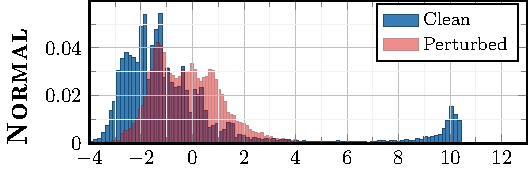
\includegraphics[height=1.35cm]{c10_q81auunfp_nt_original_logits.pdf}
	\end{subfigure}
	\begin{subfigure}{0.12\textwidth}
		\vspace*{0px}
		
		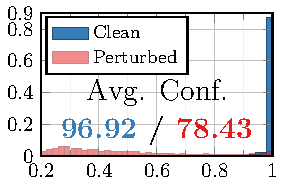
\includegraphics[height=1.425cm]{c10_q81auunfp_nt_original_confidences.pdf}
	\end{subfigure}
	\begin{subfigure}{0.12\textwidth}
		\vspace*{0px}
		
		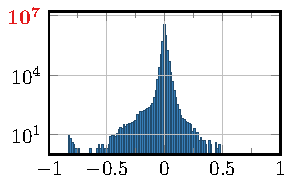
\includegraphics[height=1.425cm]{c10_q81auunfp_nt_original_weights.pdf}
	\end{subfigure}
	
	\hspace*{-0.4cm}
	\begin{subfigure}{0.24\textwidth}
		\vspace*{3px}
		
		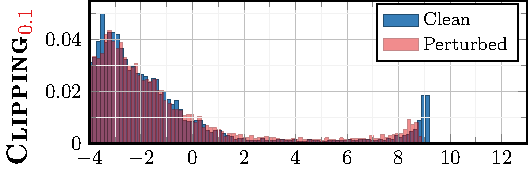
\includegraphics[height=1.35cm]{c10_q801auunfp_nt_original_logits.pdf}
	\end{subfigure}
	\begin{subfigure}{0.12\textwidth}
		\vspace*{0px}
		
		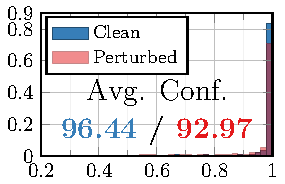
\includegraphics[height=1.425cm]{c10_q801auunfp_nt_original_confidences.pdf}
	\end{subfigure}
	\begin{subfigure}{0.12\textwidth}
		\vspace*{3px}
		
		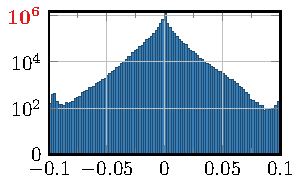
\includegraphics[height=1.425cm]{c10_q801auunfp_nt_original_weights.pdf}
	\end{subfigure}
	
	\hspace*{-0.3cm}
	{\color{black!25!white}\rule{0.5\textwidth}{0.5px}}
	
	\hspace*{-0.4cm}
	\begin{subfigure}{0.24\textwidth}
		\vspace*{0px}
		
		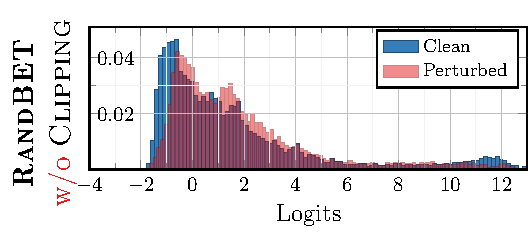
\includegraphics[height=1.825cm]{c10_q81auunrfp_sawt_bit_random_g001_pop1_logits.pdf}
	\end{subfigure}
	\begin{subfigure}{0.12\textwidth}
		\vspace*{0px}
		
		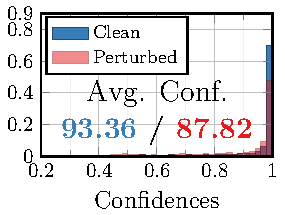
\includegraphics[height=1.7cm]{c10_q81auunrfp_sawt_bit_random_g001_pop1_confidences.pdf}
	\end{subfigure}
	\begin{subfigure}{0.12\textwidth}
		\vspace*{3px}
		
		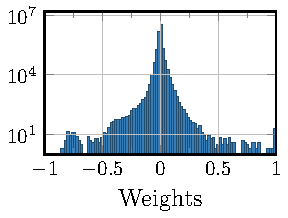
\includegraphics[height=1.7cm]{c10_q81auunrfp_sawt_bit_random_g001_pop1_weights.pdf}
	\end{subfigure}
	
	\vspace*{-8px}
	\caption{\textbf{Effect of Weight Clipping.} On \CifarT, weight clipping constraints the weights (right), thereby implicitly limiting the possible range for logits (left, {\color{colorbrewer2}blue}).
	However, even for $\wmax = 0.1$ the DNN is able to produce high confidences (middle, {\color{colorbrewer2}blue}), suggesting that more weights are used to obtain these logits. Furthermore, the impact of random bit errors, $p = 1\%$, on the logits/confidences ({\color{colorbrewer1}red}) is reduced significantly. \Random (trained with $p = 1\%$, w/o weight clipping), increases the range of weights and is less effective at preserving logit/confidence distribution. %Logit/confidence histograms normalized over $10\cdot 128$ examples.
	}
	\label{fig:clipping}
	\vspace*{-0.2cm}
\end{figure}

\textbf{Robust Quantization:} Quantization as in \eqnref{eq:quantization} does \emph{not} provide optimal robustness against bit errors. First, the floor operation $\lfloor \nicefrac{w_i}{\Delta}\rfloor$ is commonly implemented as float-to-integer conversion. Using proper rounding $\lceil\nicefrac{w_i}{\Delta}\rfloor$ instead has negligible impact on accuracy, even though approximation error improves slightly. In stark contrast, bit error robustness is improved considerably. During training, DNNs can compensate the differences in approximation errors, even for small precision $m < 8$. However, at test time,
rounding decreases the impact of bit errors considerably. Second, \eqnref{eq:quantization} uses signed integers for symmetric quantization. For asymmetric quantization, with arbitrary $[\qmin, \qmax]$, we found quantization into \emph{unsigned} integers to improve robustness, \ie, $Q : [\qmin, \qmax] \mapsto \{{\color{red}0}, \ldots, {\color{red}2^m - 1}\}$. This is implemented using an additive term of $2^{m-1}-1$ in \eqnref{eq:quantization}. While accuracy is not affected, the effect of bit errors in the sign bit changes: in symmetric quantization, the sign bit mirrors the sign of the weight value. For asymmetric quantization, an unsigned integer representation is more meaningful. Overall, our \textbf{robust fixed-point quantization (\Quant)}  uses per-layer, asymmetric quantization into unsigned integers with rounding.
These seemingly \emph{small differences} have little to no impact on accuracy, while having tremendous impact on robustness against bit errors, see \secref{subsec:experiments-quantization} and \appref{sec:supp-implementation}. 
\revision{They are simple to implement, do not add training complexity or hyper-parameters and demonstrate the importance of robustness in developing DNN quantization schemes.}

\begin{algorithm}[t]
\caption{\textbf{Random Bit Error Training (\Random).} The forward passes are performed using \blue{de-quantized weights (blue)}. Perturbed weights are obtained by injecting bit errors in the \red{quantized weights (in red)}. The update, averaging gradients from both forward passes, is performed in \magenta{floating-point (magenta)}. Also see \figref{fig:flowchart}.}
\label{alg:training}
\begin{algorithmic}[1]
\small
\Procedure{RandBET}{$p$}
    \State initialize \magenta{$w^{(0)}$}
	\For{$t = 0, \ldots, T - 1$}
    	\State sample batch $\{(x_b, y_b)\}_{b = 1}^B$
    	\State \{element-wise clipping:\}
    	\State $\magenta{w^{(t)}} = \min(\wmax, \max(-\wmax, \magenta{w^{(t)}}))$
    	\State \{quantization:\}
    	\State $\red{v^{(t)}} = Q(\magenta{w^{(t)}})$
        \State $\blue{w_q^{(t)}} = Q^{-1}(\red{v^{(t)}})$
        \State \{clean forward and backward pass:\}
        \State $\Delta^{(t)} = \nabla_w \sum_{b = 1}^B \mathcal{L}(f(x_b; \blue{w_q^{(t)}}), y_b)$
        \State \{\emph{perturbed} forward and backward pass:\}
        \State $\blue{\tilde{w}_q^{(t)}}{\hskip 1px=\hskip 1px}Q^{-1}(\biterror_p(\red{v^{(t)}}))$\label{line:attack} \{inject random bit errors\}
        \State $\tilde{\Delta}^{(t)} = \nabla_w \sum_{b = 1}^B \mathcal{L}(f(x_b; \blue{\tilde{w}_q^{(t)}}), y_b)$
        \State \{average gradients and weight update:\}
        \State $\magenta{w^{(t + 1)}} = \magenta{w^{(t)}} - \gamma(\Delta^{(t)} + \tilde{\Delta}^{(t)})$
    \EndFor
    \State \textbf{return} $\blue{w_q^{(T)}} = Q^{-1}(Q(\magenta{w^{(T)}}))$
\EndProcedure
\end{algorithmic}
\end{algorithm}

\subsection{Training with Weight Clipping as Regularization}
\label{subsec:robustness-clipping}

\textbf{Weight clipping} refers to constraining the weights to $[-\wmax, \wmax]$ \emph{during training}, where $\wmax$ is a hyper-parameter. Generally, $\wmax$ is independent of the quantization range(s) which always adapt(s) to the weight range(s) at hand. However, weight clipping limits the maximum possible quantization range (\cf \secref{subsec:robustness-quantization}), \ie, $\qmax \leq \wmax$.
It might seem that weight clipping with small $\wmax$ automatically improves robustness against bit errors as the absolute errors are reduced. However, the \emph{relative} errors are not influenced by rescaling. As the DNN's decision is usually invariant to rescaling, reducing the scale of the weights does not impact robustness. In fact, the mean relative error of the weights in \figref{fig:quantization} (right) increased with clipping at $\wmax = 0.1$. Thus, weight clipping does \emph{not} ``trivially'' improve robustness by reducing the scale of weights. Nevertheless, we found that weight clipping actually improves robustness considerably on top of our robust quantization.

The interplay of weight clipping and minimizing the the cross-entropy loss during training is the key. High confidences can only be achieved by large differences in the logits. Because the weights are limited to $[-\wmax, \wmax]$, large logits can only be achieved using more weights in each layer to produce larger outputs. This is illustrated in \figref{fig:clipping} (right): using $\wmax = 0.1$, the weights are (depending on the layer) up to $5$ times smaller. Considering deep NNs, the ``effective'' scale factor for the logits is significantly larger, scaling exponentially with the number of layers. Thus, using $\wmax = 0.1$ is a significant constraint on the DNNs ability to produce large logits. As result, weight clipping produces a much more uniform weight distribution.
\figref{fig:clipping} (left and middle) shows that a DNN constrained at $\wmax = 0.1$ can produce similar logit and confidence distributions (in {\color{colorbrewer2}blue}) as the unclipped DNN. At the same time, random bit errors, have a significantly smaller impact on the logits and confidences (in {\color{colorbrewer1}red}). \figref{fig:clipping} (right column) also shows the induced redundancy in the weight distribution. Weight clipping leads to more weights being utilized, \ie, less weights are zero (note log-scale, marked in {\color{colorbrewer1}red}, on the y-axis). Also, more weights reach large values, relative to the maximum absolute weight. Overall, we found weight clipping to be an easy-to-use but effective measure to improve weight robustness. We use \Clipping[$\wmax{=}0.1$] to refer to, \eg, weight clipping with $\wmax = 0.1$. For more evidence supporting our argumentation, see \tabref{tab:clipping-robustness}. For example, we show that DNNs loose robustness when using label smoothing, \ie, not enforcing high confidences/logits during training.
\revision{Finally, weight clipping is straight-forward to implement (\cf \algref{alg:training}, line 6) and adds negligible training cost. The additional hyper-parameter, \ie, $\wmax$, can easily be tuned based on constraints on clean (or robust) performance, \cf \secref{subsec:experiments-clipping}.}

\subsection{Random Bit Error Training (\Random)}
\label{subsec:robustness-training}

In \emph{addition to} weight clipping and robust quantization, we inject random bit errors with probability $p$ during training to further improve robustness. This results in the following learning problem, which we optimize as illustrated in \figref{fig:flowchart}:
\begin{align}
	\begin{split}
    	&\min_w \mathbb{E}[\mathcal{L}(f(x; \tilde{w}), y) + \mathcal{L}(f(x; w), y)]\\
    	\text{s.t.}&\quad v = Q(w),\, \tilde{v} = \biterror_p(v),\, \tilde{w} = Q^{-1}(\tilde{v}).
   	\end{split}\label{eq:random-training-average}
\end{align}
where $(x, y)$ are labeled examples, $\mathcal{L}$ is the cross-entropy loss and $v = Q(w)$ denotes the (element-wise) quantized weights $w$ which are to be learned. $\biterror_p(v)$ injects random bit errors with rate $p$ in $v$. Note that we consider both the loss on clean weights and weights with bit errors. This is desirable to avoid an increase in (clean) test error and stabilizes training compared to training only on bit errors in the weights. Note that bit error rate $p$ implies, in expectation, $pmW$ bit errors. Following \algref{alg:training}, we use stochastic gradient descent to optimize \eqnref{eq:random-training-average}, by performing the gradient computation using the perturbed weights $\tilde{w} = Q^{-1}(\tilde{v})$ with $\tilde{v} = \biterror_p(v)$, while applying the gradient update on the (floating-point) clean weights $w$. In spirit, this is similar to data augmentation, however, the perturbation is applied on the weights instead of the inputs. As we found that introducing bit errors right from the start may prevent the DNN from converging, we apply bit errors as soon as the (clean) cross-entropy loss is below $1.75$. Interestingly, weight clipping and \Random have somewhat orthogonal effects, which allows to combine them easily in practice: While weight clipping encourages redundancy in weights by constraining them to $[-\wmax,\wmax]$, % and activations, 
\Random (w/o weight clipping) causes the DNN to have larger tails in the weight distribution, as shown in \figref{fig:clipping} (bottom). However, considering logits and confidences, especially with random bit errors (in {\color{colorbrewer1}red}), \Random alone performs slightly worse than \Clipping[$0.1$]. Thus, \Random becomes particularly effective when combined with weight clipping, as we make explicit using the notation \Random[$\wmax$] in \algref{alg:training}.
\revision{While \Random increases training complexity (\cf \algref{alg:training}), inference is \emph{not} affected. This is in stark contrast to hardware- or redundancy-based bit error mitigation strategies which usually impact inference time and energy consumption. We also note that the additional hyper-parameter, \ie, $p$, is easily chosen according to the target bit error rate.}